\chapter[Sprint 3]{Study and Implementation of Sprint 3: Diagram \& Workspace Management}

\section{Introduction}
Sprint 3 focuses on implementing core diagram and workspace management functionality, representing a significant milestone in developing a comprehensive diagramming tool. This sprint delivers diagram lifecycle management and advanced workspace features including AI-assisted editing and interactive code editing capabilities.

\section{Sprint Planning}

\subsection{Objectives}
Primary objectives include implementing comprehensive diagram CRUD operations, establishing robust workspace environment with split-view functionality, integrating AI assistance for diagram editing, and ensuring seamless PlantUML server integration for rendering.

\subsection{Sprint Backlog}

\begin{table}[h]
    \centering
    \begin{tabular}{|c|l|c|p{8cm}|c|}
    \hline
    \textbf{ID} & \textbf{Feature} & \textbf{Sub-ID} & \textbf{User Story} & \textbf{Priority} \\
    \hline
    4 & Manage Diagrams & 4.1 & As a user; I want to create a new diagram. & M \\
    \hline
      &  & 4.2 & As a user; I want to view my diagram. & M \\
    \hline
      &  & 4.3 & As a user; I want to update diagram details. & M \\
    \hline
      &  & 4.4 & As a user; I want to delete a diagram. & M \\
    \hline
    5 & Manage Workspace & 5.1 & As a user; I want to edit diagram code in an interactive editor. & M \\
    \hline
      &  & 5.2 & As a user; I want to chat with an AI model to edit diagram code. & C \\
    \hline
      &  & 5.3 & As an AI system; I need to respond to user requests and help edit diagram code. & C \\
    \hline
      &  & 5.4 & As a PlantUML Server; I need to render diagram code into diagram images. & M \\
    \hline
    \end{tabular}
    \caption{Manage Diagrams and Workspace User Stories Requirements Table}
    \label{tab:diagrams_workspace}
    \end{table}
\section{System Analysis}

\subsection{Use Case Overview}

\begin{figure}[H]
\centering
\includegraphics[width=0.75\textwidth]{conception/SprintIV/use_case_diagrams/use_case_diagram_of_SprintIV.png}
\caption{Sprint 3 Use Case Diagram}
\end{figure}

\subsection{Core Features}

\subsubsection{Diagram Management}
\begin{figure}[H]
\centering
\includegraphics[width=0.7\textwidth]{conception/SprintIV/use_case_diagrams/refined_use_case_feature_diagram_management.png}
\caption{Diagram Management Use Cases}
\end{figure}

Key operations include:
\begin{itemize}
    \item \textbf{Create Diagram}: User initiates new diagram creation with name and type selection
    \item \textbf{View Diagram}: Interactive editor with real-time preview and validation
    \item \textbf{Delete Diagram}: Secure deletion with confirmation dialog
\end{itemize}

\subsubsection{Workspace Management}
\begin{figure}[H]
\centering
\includegraphics[width=1\textwidth]{conception/SprintIV/use_case_diagrams/refined_use_case_feature_workspace_management.png}
\caption{Workspace Management Use Cases}
\end{figure}

Core workspace features:
\begin{itemize}
    \item \textbf{Edit Diagram}: Interactive code editor with syntax highlighting
    \item \textbf{AI Chat}: Natural language assistance for diagram creation and troubleshooting
    \item \textbf{Save Changes}: Persistent storage with validation and error handling
\end{itemize}

\section{Sequence Diagrams}

% \subsection{Process Flow}
% \begin{figure}[H]
% \centering
% \includegraphics[width=0.75\textwidth]{conception/SprintIV/Activity_diagrams/edit_diagams.png}
% \caption{Diagram Editing Activity Flow}
% \end{figure}

\subsection{Diagram Creation Process}

\begin{figure}[H]
\centering
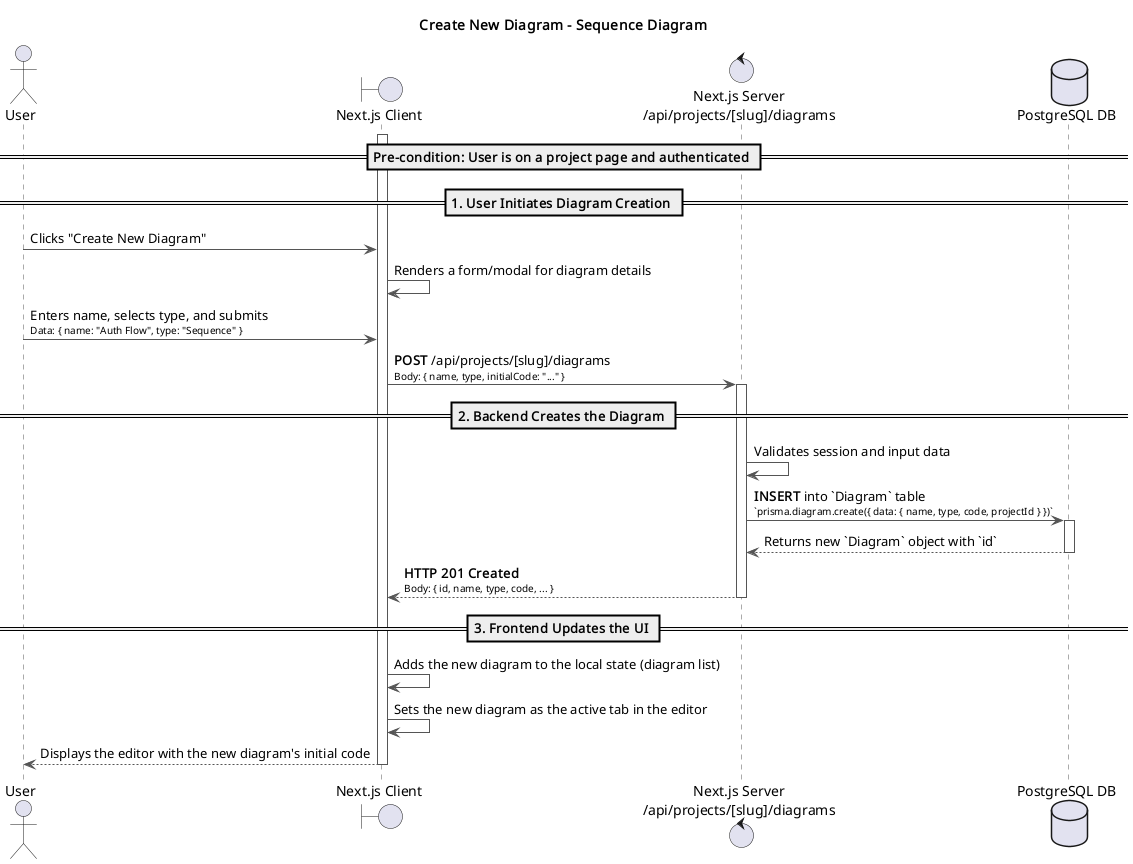
\includegraphics[width=1\textwidth]{conception/SprintIV/sequence_diagrams/sequence_diagramManagement_4_1_CreateNewDiagram.png}
\caption{Create New Diagram Sequence}
\end{figure}

\subsection{AI-Assisted Editing}
\begin{figure}[H]
\centering
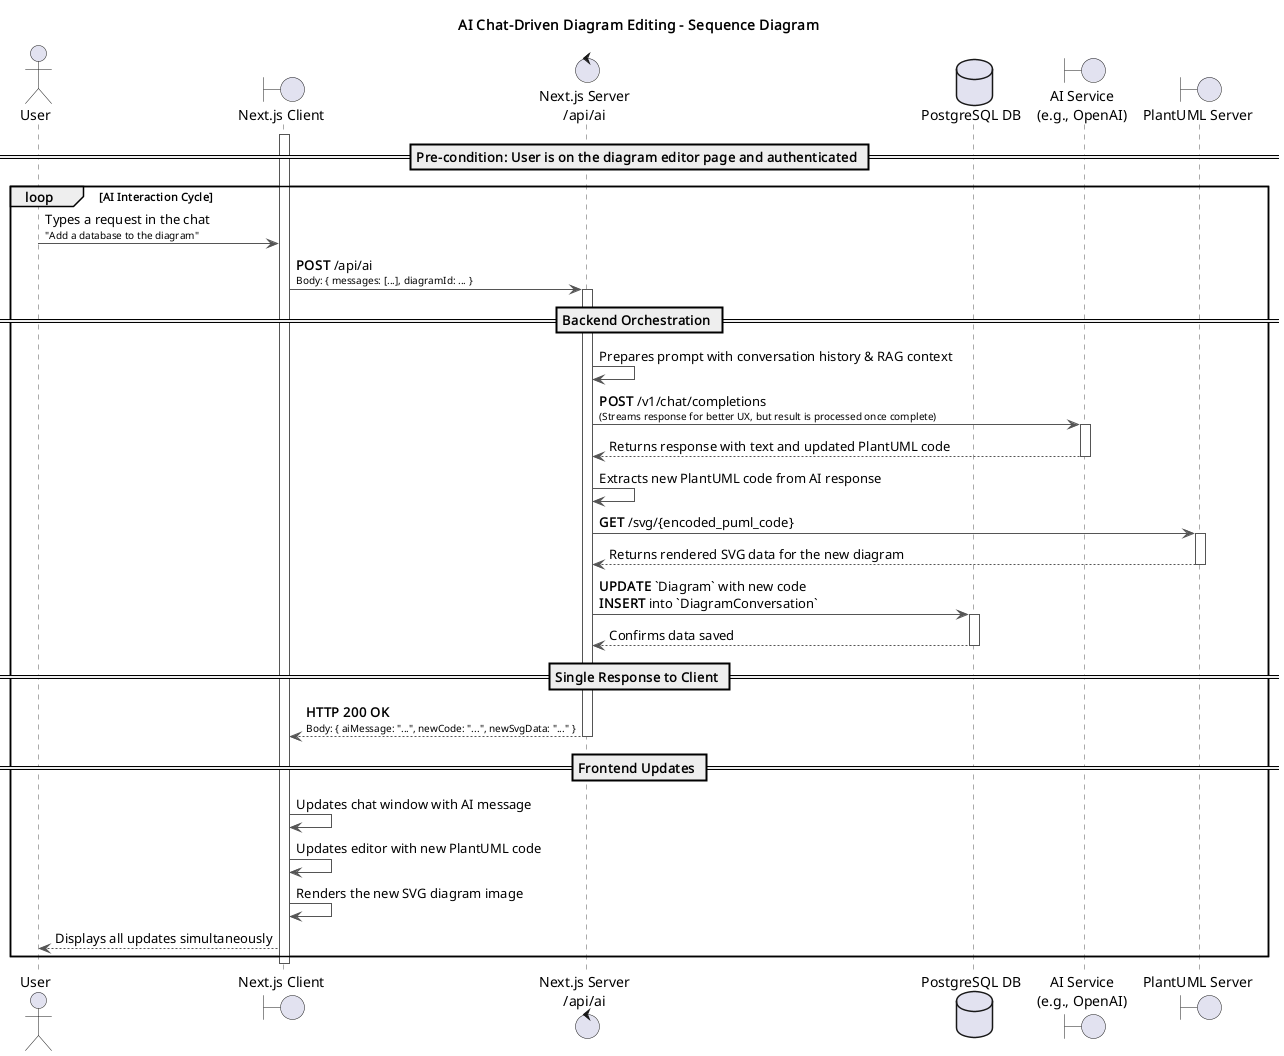
\includegraphics[width=0.8\textwidth]{conception/SprintIV/sequence_diagrams/sequence_workspaceManagement_5_3_ChatWithAIMode.png}
\caption{AI Chat Integration Sequence}
\end{figure}

\section{Implementation Results}

\subsection{Core Interfaces}

\begin{figure}[H]
\centering
\includegraphics[width=0.6\textwidth]{screenshots/add-diagram.png}
\caption{Diagram Creation Interface}
\end{figure}

The diagram creation interface provides intuitive name specification, type selection, and project initialization capabilities.

\begin{figure}[H]
\centering
\includegraphics[width=1\textwidth]{screenshots/code-editor.png}
\caption{Interactive Code Editor with Real-time Preview}
\end{figure}

The interactive workspace features syntax highlighting, real-time validation, and seamless preview integration for enhanced productivity.

\begin{figure}[H]
\centering
\includegraphics[width=0.8\textwidth]{screenshots/AI-assistant.png}
\caption{AI Assistant Integration}
\end{figure}

AI assistant provides intelligent support through natural language interaction for diagram creation, code improvement, and troubleshooting assistance.

\subsection{Workspace Environment}


\begin{figure}[H]
\centering
\includegraphics[width=0.8\textwidth]{screenshots/edit-diagram-project-2.png}
\caption{Split-View Workspace - Secondary View}
\end{figure}

The dual-pane workspace enables simultaneous code editing and diagram preview, providing immediate visual feedback and significantly improving user productivity.

\section{Sprint Retrospective}

\subsection{Achievements}
\begin{itemize}
    \item Successfully implemented complete diagram CRUD operations
    \item Effective AI assistant integration with natural language processing
    \item Smooth PlantUML server integration for high-quality rendering
    \item Real-time editing with immediate visual feedback
\end{itemize}

\subsection{Challenges}
\begin{itemize}
    \item AI service integration complexity
    \item Performance optimization for large diagrams
\end{itemize}



\section{Conclusion}

Sprint 3 successfully delivered comprehensive diagram and workspace management capabilities that form the application's core foundation. The implementation combines efficient CRUD operations with intelligent AI assistance and interactive editing features, providing users with a powerful and intuitive diagramming platform. The integration of PlantUML server ensures high-quality rendering, while the AI assistant adds significant value for complex diagramming tasks. These achievements establish a solid foundation for future enhancements and advanced features in subsequent development cycles.